\section{Worked examples}\label{sec:examples}

The paper uses seven worked examples as an end-to-end smoke test of the
validated core rather than as seven miniature empirical papers. Each
example has an executable script under \code{Paper-JSS/replication/}
that writes JSON, table fragments, and any figures used by the build.
The examples cover the identification strategies an applied
econometrician is most likely to ask a unified \proglang{Python}
front end to handle: selection on observables, IV, staggered DiD, RD,
synthetic control, machine-learning treatment-effect estimation,
matching, causal time-series counterfactuals, and -- the case that
reaches across all three ecosystems -- panel counterfactual estimators
and interaction effects run on the same bytes in \proglang{Python},
\proglang{R}, and \proglang{Stata}.

The non-trivial workflow case study is the \code{mpdta} staggered-DiD
example: it moves from design-specific estimation to aggregation,
event-study inspection, Honest-DiD sensitivity, Bacon decomposition,
citations, and export from the same fitted objects. The other examples
are shorter stress tests around the same contract, especially where a
reference package, public data extract, or known-truth simulation gives a
clean validation target.
Table~\ref{tab:worked-example-map} maps those examples to the
replication scripts and validation facts used by the paper.

\begin{table}[!ht]
\centering\scriptsize
\begingroup
\setlength{\tabcolsep}{3pt}
\begin{tabular}{@{}p{0.16\linewidth}p{0.20\linewidth}p{0.27\linewidth}p{0.23\linewidth}@{}}
\toprule
Example & \statspai{} surface exercised & Headline validation fact & Replication artifact \\
\midrule
Card (1995) & \code{sp.regress}, \code{sp.iv}, \code{sp.dml}, forest &
OLS and 2SLS match \proglang{R} on \code{wooldridge::card} at machine precision; DML/forest are reported as stochastic ML checks. &
\code{ex01\_card.py}; original-data module \code{01\_card} \\
Basque (2003) & \code{sp.synth}, sensitivity &
ADH special-predictor specification on the original bytes gives post-1970 gap \(-0.8946\) vs \proglang{R} \(-0.8944\) vs \proglang{Stata} \(-0.8943\); default \(V\)-choice is disclosed separately. &
\code{ex02\_basque.py}; original-data module \code{03\_basque} \\
\texttt{mpdta} staggered DiD & CS, aggregation, Honest-DiD, Bacon &
Simple ATT matches \pkg{did} and \code{csdid} to machine precision on the calibrated replica bytes, and matches \pkg{did} at \(2.3\times10^{-14}\) on the original \code{did::mpdta} bytes. &
\code{ex03\_csdid.py}; module \code{04\_csdid} \\
Lee (2008) RD & RD robust and density diagnostics &
The native CCT bandwidth and robust estimate match \pkg{rdrobust} on the RDsenate extract to \(3\times10^{-13}\); the official \pkg{rdrobust} \proglang{Python} port agrees with the native path. &
\code{ex04\_lee.py}; modules \code{06\_rd}, \code{09\_rddensity} \\
LaLonde / Dehejia--Wahba & OLS, PSM, IPW, balance diagnostics &
Original public extracts from \pkg{MatchIt} and \pkg{causalsens} match \proglang{R}; the observational design preserves the classic sign/bias warning. &
\code{ex05\_lalonde.py}; original-data modules \code{04}, \code{04b} \\
Advertising lift & \code{sp.causal\_impact} &
Known simulated lift \(=4.2\) is recovered at \(4.306\) with the 95\% interval containing truth and pre-period RMSE below the registered guard. &
\code{ex06\_causal\_impact.py} \\
fect / interflex & \code{sp.panel\_view}, \code{sp.fect}, \code{sp.interflex} &
Three fect outcome models and three interflex estimators return the same numbers as \proglang{R} \pkg{fect} / \pkg{interflex} and the authors' \proglang{Stata} commands on identical bytes (worst relative gap \(10^{-9}\)). &
\code{ex08\_fect\_interflex.py}; modules \code{86\_fect}, \code{87\_interflex} \\
\bottomrule
\end{tabular}
\endgroup
\caption{Worked-example coverage and replication artifacts. Each row is
reproduced by the named script under \code{Paper-JSS/replication/}; the
main text keeps to the executable contract and the headline validation
fact, while full per-row provenance lives in the replication archive.}
\label{tab:worked-example-map}
\end{table}

\subsection{Card (1995): returns to schooling}\label{sec:ex-card}

The Card workflow \citep{card1995using} loads the NLSYM extract, fits
OLS, 2SLS, DML, and a causal forest through the same
\code{(y, X, data)} contract, and exports the resulting table with
\code{sp.regtable}. \code{sp.datasets.card\_1995()} returns the public
\code{wooldridge::card} extract itself, so the session of
Listing~\ref{lst:motivating} runs on the original bytes;
Listing~\ref{lst:card-output} continues that session at a prompt and
prints what it produces.

\Needspace*{30\baselineskip}
\begin{lstlisting}[caption={The session of
Listing~\ref{lst:motivating}, continued at a prompt: three result
classes render into one table, and \code{sp.audit} separates the checks
this fit has passed, still lacks, or cannot have. Printed with
\code{rules="ascii"} so the transcript is byte-safe on any console
code page.},label={lst:card-output},captionpos=b]
>>> print(sp.regtable(ols, iv, dml, keep=["educ", "ATE"], stars=True,
...                   model_labels=["OLS", "2SLS", "DML PLR"],
...                   rules="ascii"))
==============================================================
                             OLS          2SLS       DML PLR
==============================================================
educ                   0.0740***     0.1323***
                        (0.0035)      (0.0492)

ATE                                                0.0741***
                                                    (0.0037)

==============================================================
First-stage F                            16.72
==============================================================
N                          3,010         3,010         3,010
R2                         0.291         0.225
Adj. R2                    0.289
F                        204.932
==============================================================
Standard errors in parentheses
*** p<0.01, ** p<0.05, * p<0.10
>>> print(sp.audit(iv))
Reviewer audit: IV-2SLS [iv]
1 of 2 applicable checks satisfied (passed 1, failed 0, missing 1; 1 n/a)

  passed  weak_instrument         value 16.72 vs threshold 10
  n/a     overid_test             just-identified; no restriction to test
  missing anderson_rubin_ci       run sp.anderson_rubin_ci

Missing checks are evidence a reviewer will expect, not errors.
n/a checks do not exist for this fit and are not counted.
\end{lstlisting}

The three linear-in-\code{educ} summaries land where the literature
puts them: \(\hat\beta_{\mathrm{OLS}} = 0.07401\) against Card's
published 0.075, and
\(\hat\beta_{\mathrm{IV}}^{\mathrm{nearc4}} = 0.1323\) against his
0.132, reproducing the IV-above-OLS pattern that motivates the design;
cross-fit DML agrees with OLS to the third decimal. \proglang{R}'s
\code{lm}+\pkg{sandwich} and \pkg{AER}\code{::ivreg} return the same
two coefficients on the same CSV bytes at relative errors
\(7.9\times 10^{-15}\) and \(1.6\times 10^{-11}\)
(Table~\ref{tab:headline-parity}). The \code{sp.audit} block is the
audit-hook claim made concrete, and it distinguishes three states that a
flat checklist conflates. The first-stage \(F\) of 16.72 clears the
\(F>10\) rule of thumb \citep{staiger1997instrumental,stock2005testing};
``passed'' means only that this screen was met --- it is neither a test
of instrument validity nor a guarantee against weak-instrument
distortion, which is why weak-instrument-robust Anderson--Rubin inference
is still listed as missing. The over-identification test is reported as
not applicable rather than missing: with one endogenous regressor and one
excluded instrument the model is just-identified, the Sargan/Hansen
statistic has zero degrees of freedom, and there is no restriction to
test. The audit reads the instrument and endogenous-regressor counts from
the fitted object to decide this; when an over-identified fit already
carries a \(J\) statistic it is read and graded, and the text, JSON, and
MCP outputs carry the same \code{not\_applicable} status and reason.

The four estimators do not share one identification argument, and the
table should not be read as four estimates of one parameter. The 2SLS
coefficient uses \code{nearc4} as an excluded instrument and, with
heterogeneous returns, identifies a local average effect for
instrument-compliers under relevance, exclusion, independence, and
monotonicity. The DML and forest calls in Listing~\ref{lst:motivating}
use no instrument: they adjust for the listed covariates and are causal
only under conditional exogeneity of schooling, the assumption the IV
design exists to avoid. On these data they therefore estimate an
adjusted partial association, and the forest's heterogeneity is
heterogeneity in that association. The listing shows that the four fits
share one result contract; it does not identify heterogeneous returns to
schooling, which would require an IV-based heterogeneity estimator and
its own validation. With that caveat, Listing~\ref{lst:card-cate}
summarises the fitted forest's conditional effects.

\Needspace*{14\baselineskip}
\begin{lstlisting}[caption={How far the return to schooling varies
across the sample, from the forest fitted in
Listing~\ref{lst:motivating}. With \pkg{grf}'s honest, 2{,}000-tree
defaults the interquartile range spans roughly 6.3\% to 8.6\% per year
around a mean of 7.7\%, as \proglang{R} \pkg{grf} finds on the same
bytes (6.3\% to 8.7\% around 7.6\%): the estimated dispersion is
modest, about a fifth of the 0.081 standard deviation the pre-1.29.0
forest engine reported for the same call on the same
data.},label={lst:card-cate},captionpos=b]
>>> print(sp.cate_summary(cf).loc[["Mean (ATE)", "Std. Dev.",
...                                "Q25", "Q75"]].round(4))
              CATE
Mean (ATE)  0.0765
Std. Dev.   0.0164
Q25         0.0633
Q75         0.0859
\end{lstlisting}


Two boundaries are worth stating here because the rest of
Section~\ref{sec:parity} depends on them. First, the Track~A parity
fixture for this design is a \emph{calibrated replica}, not the extract
above: it is a redistribution-safe guard that preserves the
IV-greater-than-OLS pattern, which is why the Card rows of
Table~\ref{tab:track-a-cross-language-snapshot} carry different coefficients from the
original-data rows of Table~\ref{tab:headline-parity}. Second, the
treatment here is years of schooling, a continuous variable, so the
forest's scalar aggregate is the average partial effect built from the
continuous-treatment debiased score rather than the binary AIPW
aggregate that the Track~B forest row validates
(Section~\ref{sec:track-b}). On these bytes
\code{cf.average\_treatment\_effect()} returns \(0.0787\) (SE
\(0.0049\)), as does \pkg{grf}~2.6.1 (\(0.0787\), SE \(0.0049\)); the
two single fits differ by \(1\times10^{-5}\), which is one draw from
each engine rather than a grade (Section~\ref{sec:validation-tiers});
both packages refuse the ATT and ATC targets for a continuous
treatment. Both artifacts are rebuilt by
\code{replication/scripts/ex01\_card.py}; the \pkg{grf} side by
\code{ex01\_card\_grf.R}.

\subsection{Abadie--Gardeazabal (2003): the Basque country}\label{sec:ex-basque}

The Basque example \citep{abadie2003economic} exercises the
synthetic-control dispatcher and the post-estimation sensitivity hooks.
The publication-critical point is that the paper does not hide SCM
non-uniqueness behind a loose tolerance: under the canonical
Abadie--Diamond--Hainmueller \citep{abadie2010synthetic} setup used by
\code{Synth::synth} -- one special predictor per pre-treatment year and
nested \(V\) optimization -- and on the \emph{original}
\code{Synth::basque} bytes, \statspai{} returns an average post-1970
GDPpc gap of \(-0.8946\), \proglang{R} returns \(-0.8944\), and Stata
\code{synth} returns \(-0.8943\); all pairwise gaps are within
\(4\times 10^{-4}\), and all three lie near the
published \(-0.855\) anchor. On the calibrated Basque replica of the
Track~A harness the same specification instead splits the references by
\(2.3\times10^{-2}\); Section~\ref{sec:scm-identification} reports both
facts as the paper's non-uniqueness disclosure. The package default
\code{sp.synth(method="classic")}, which sets \(V=I\) when only the
pre-treatment outcome path is used as the predictor vector, remains a
documented default convention rather than a hidden failed parity row.
Figure~\ref{fig:basque-gap} makes that default-convention boundary
visible as a gap path rather than a scalar discrepancy.

\begin{figure}[!ht]\centering
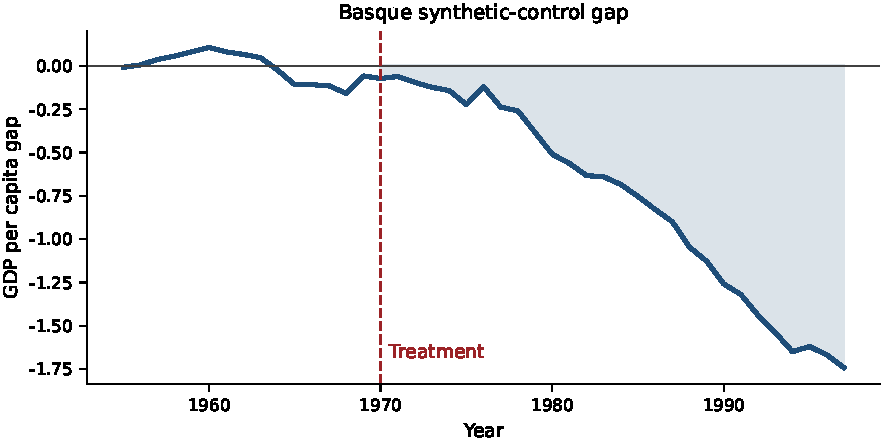
\includegraphics[width=\textwidth]{figures/ex02_basque_gap.pdf}
\caption{Synthetic-control gap (treated minus synthetic per-capita GDP)
for the Basque country under the package-default
\code{sp.synth(method="classic")} path (\(V=I\), outcome-path
predictors) on the calibrated Basque replica, with the
1970 treatment marked. This is the default-convention illustration, not
the ADH parity specification of the parity tables: the parity numbers
come from the special-predictor, nested-\(V\) setup reported in
Section~\ref{sec:scm-identification}. Regenerated by
\code{replication/scripts/generate\_figures.py}; numerical artifacts are
written by \code{replication/scripts/ex02\_basque.py}.}
\label{fig:basque-gap}
\end{figure}

\subsection[Callaway-Sant'Anna staggered DiD: mpdta]{Callaway--Sant'Anna staggered DiD: \texttt{mpdta}}\label{sec:ex-csdid}

The \code{mpdta} example is the main panel-workflow demonstration;
Listing~\ref{lst:csdid} shows the full fit-to-sensitivity chain from one
fitted object.

\begin{lstlisting}[caption={Callaway--Sant'Anna fit, simple- and
event-study aggregation, Rambachan--Roth Honest-DiD bounds, and the
Goodman--Bacon decomposition --- all from the same fitted
object.},label={lst:csdid},captionpos=b]
mpdta = sp.datasets.mpdta()
cs  = sp.callaway_santanna(mpdta, y="lemp", t="year", i="countyreal",
                           g="first_treat", control_group="nevertreated",
                           estimator="reg")
agg = sp.aggte(cs, type="simple", random_state=0)
es  = sp.aggte(cs, type="dynamic", random_state=0)
hd  = sp.honest_did(cs, e=0, method="smoothness")
bd  = sp.bacon_decomposition(mpdta, y="lemp", treat="treat",
                             time="year", id="countyreal")
\end{lstlisting}

\code{sp.callaway\_santanna} estimates group-time ATTs,
\code{sp.aggte} reports simple and dynamic aggregations,
\code{sp.honest\_did} applies the Rambachan--Roth sensitivity
post-estimator, and \code{sp.bacon\_decomposition} gives the TWFE
weight diagnostic \citep{goodmanbacon2021difference}.
Listing~\ref{lst:csdid-output} prints the two objects a reader of this
literature would want to see: the aggregated effect, and how much
parallel-trends violation it survives.

\Needspace*{16\baselineskip}
\begin{lstlisting}[caption={The simple aggregation and the
Rambachan--Roth smoothness bounds from the fit of
Listing~\ref{lst:csdid}. \code{M} is the bound on how much the
post-treatment trend may deviate from the linear extrapolation of the
pre-treatment trend; \code{rejects\_zero} is whether the robust
confidence set still excludes zero at that
bound.},label={lst:csdid-output},captionpos=b]
>>> print(f"{float(agg.estimate):.6f}  {float(agg.se):.6f}")
-0.032977  0.007961
>>> print(hd.round(4).to_string(index=False))
     M  ci_lower  ci_upper  rejects_zero
0.0000   -0.0546   -0.0214          True
0.0037   -0.0566   -0.0129          True
0.0074   -0.0582   -0.0017          True
0.0112   -0.0601    0.0058         False
0.0149   -0.0632    0.0106         False
0.0223   -0.0706    0.0180         False
\end{lstlisting}

The reading is the one \citet{rambachan2023more} intend: the
first-period effect is robust to a post-treatment trend deviation of up
to about \code{M} \(= 0.0074\) log points, and the confidence set
admits zero once the allowed deviation reaches \(0.0112\). That
breakdown value, not the pre-trend test's \(p\)-value, is the quantity
a referee should be given, and it comes off the same fitted object as
the point estimate.

That last clause is the case for the shared contract, and it can be
measured. The Rambachan--Roth interval needs the \emph{joint} covariance
of the event-study coefficients, the relative times, and the position of
the reference period. Composed by hand, the workflow extracts these from
one package's aggregation object and re-enters them into another's
sensitivity function; the tempting shortcut is to rebuild the covariance
from the reported standard errors. On \texttt{mpdta} the pre- and
post-period coefficients are correlated up to 0.61, and the shortcut is
not innocuous: with \(\operatorname{diag}(\mathrm{SE}^2)\) in place of the
joint covariance the breakdown value rises from 0.0080 to 0.0101, so the
estimate would be reported as surviving trend deviations 26\% larger
than the data support, and the \(M=0\) interval shifts from
\([-0.0546,-0.0214]\) to \([-0.0477,-0.0156]\). In \statspai{},
\code{sp.honest\_did} reads the joint covariance, the relative times, and
the aggregation weights from the fitted object through one extractor,
\code{sp.event\_study\_vcov}, shared by nine event-study estimators; when
a fit cannot supply a joint covariance it says so and falls back to a
labelled approximation rather than fabricating one from standard errors.
The single entry point also means a correctness fix applies once: the
1.30.0 repair of the cohort-share term in that covariance
(Table~\ref{tab:correctness-history}) reached every estimator's
sensitivity analysis at the same time. The saving is not lines of code;
it is that the covariance, the reference period, and the estimand
travel with the estimate instead of being re-typed. The \code{random\_state=0} in
Listing~\ref{lst:csdid} is not decoration: \code{sp.aggte} follows
\pkg{did} in defaulting to a 1{,}000-draw multiplier bootstrap, so the
aggregated standard error is a random quantity and a printed
transcript of it is only reproducible once the draw is pinned. The
parity
evidence sits on two data sets, and the paper keeps them apart. On the
calibrated \texttt{mpdta} replica of Track~A module 04,
\statspai{}, \pkg{did}, and \code{csdid} all return the simple ATT
\(-0.0329765\) in the R-joined harness and agree within the registered
iterative tolerance on the analytic SE. On the \emph{original}
\code{did::mpdta} bytes, \statspai{} and \pkg{did} return the simple
ATT \(-0.03995\) at relative error \(2.3\times10^{-14}\) and the
vignette-printed overall dynamic ATT \(-0.0772\) at
\(1.6\times10^{-14}\) (Table~\ref{tab:headline-parity}). The
homogeneous calibrated
replica additionally checks that Callaway--Sant'Anna, Sun--Abraham
\citep{sun2021estimating}, BJS/imputation \citep{borusyak2024revisiting},
and DR-DiD \citep{santanna2020doubly} collapse to the same estimand when
their identification restrictions coincide.
Figure~\ref{fig:mpdta-es} is the printed event-study counterpart to
Listing~\ref{lst:csdid}.

\begin{figure}[!ht]\centering
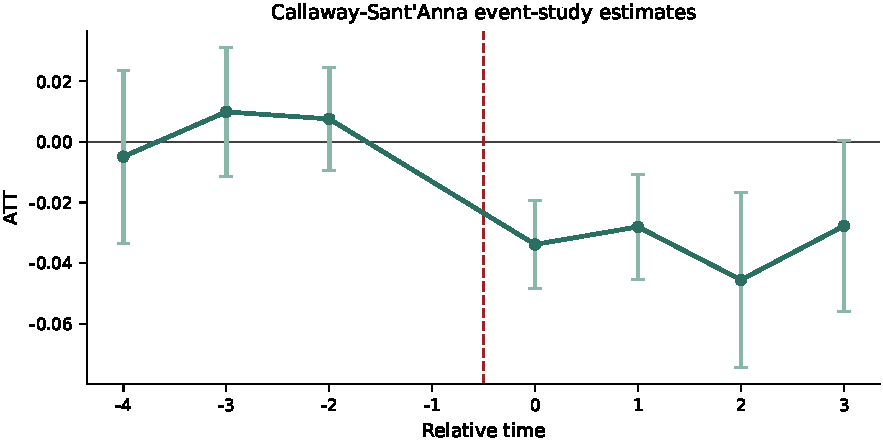
\includegraphics[width=\textwidth]{figures/ex03_mpdta_event_study.pdf}
\caption{Callaway--Sant'Anna dynamic event study on \texttt{mpdta}
(\code{sp.aggte(cs, type="dynamic")}): event-time ATTs with
simultaneous confidence bands. Regenerated by
\code{replication/scripts/generate\_figures.py}; numerical artifacts are
written by \code{replication/scripts/ex03\_csdid.py}.}
\label{fig:mpdta-es}
\end{figure}

\subsection[RD incumbency advantage (Lee-style sharp design)]{Regression discontinuity: the incumbency advantage (Lee-style sharp design)}\label{sec:ex-rd}

The RD example deliberately separates the local-polynomial estimator
from the bandwidth selector, and it keeps two data objects distinct to
avoid over-claiming. The \emph{exact} cross-language parity anchor is
the public \code{rdrobust::RDsenate} extract --- the U.S.\ Senate
margin-of-victory sample distributed with \pkg{rdrobust}, a Lee-style
sharp RD but \emph{not} \citet{lee2008randomized}'s original House
data, which we do not redistribute. The calibrated
\code{lee\_2008\_senate()} replica is a redistribution-safe
drift-guard, not a parity target: on it \code{sp.rdrobust} returns a
robust jump of \(0.0763\), and the external test only asserts that the
estimate stays in the \([0.05,0.12]\) structural neighbourhood.
On the RDsenate extract the native \code{sp.rdrobust} default, which
implements the \citet{calonico2014robust} CCT bandwidth cascade and
robust bias-corrected inference in \statspai{} itself
\citep[software article:][]{calonico2015rdrobust}, returns the same
MSE-optimal bandwidth (17.7544) and conventional and robust estimates as
\proglang{R}'s default \pkg{rdrobust} at relative error below
\(3\times10^{-13}\) (Section~\ref{sec:track-a}). Users who prefer the
authors' own code can call \code{sp.rdrobust(..., bwselect="cct")},
which delegates to the official \pkg{rdrobust} \proglang{Python} port;
the two agree to \(2\times10^{-13}\), and that agreement is recorded as
a convergence check rather than counted as parity. The previous
density-test selector gap is closed by the native \code{sp.rddensity}
port (Section~\ref{sec:track-a}).

\subsection{LaLonde (1986) / Dehejia--Wahba (1999): the NSW programme}\label{sec:ex-lalonde}

The LaLonde \citep{lalonde1986evaluating} / Dehejia--Wahba
\citep{dehejia1999causal} workflow shows the same mature result surface
under an experimental benchmark and an observational comparison. On
\code{causalsens::lalonde.psid} \citep{blackwell2014selection}, the naive OLS ATT is
\(-\$15{,}200\) in both \statspai{} and \proglang{R}, and the
covariate-adjusted OLS ATT is \(\$751.9\) on both sides; on
\code{MatchIt::lalonde}, 1:1 nearest-neighbour PSM agrees with
\pkg{MatchIt} up to the registered caliper/default convention. The
replication script also emits balance and overlap diagnostics: the
point is not that matching fixes the benchmark, but that the platform
keeps the experimental anchor, observational bias, and preprocessing
diagnostics in one auditable pipeline.

\subsection{Causal time series: advertising lift}\label{sec:ex-causal-impact}

The causal-impact example uses a deterministic Brodersen-style
\citep{brodersen2015inferring} advertising-lift simulation rather than
proprietary marketing data.
The known post-intervention lift is \(4.2\) sales units per day;
\code{sp.causal\_impact} estimates \(4.306\) with SE \(0.140\), a 95\%
interval \([4.032,4.579]\), cumulative effect \(129.2\) against true
\(126.0\), and pre-period RMSE \(0.562\). These numbers are not
cross-language parity claims; they are known-truth guards that the
time-series counterfactual machinery, the result object, and the
publication export path are wired correctly.

\subsection{Three ecosystems, one number: panel counterfactuals and interaction effects}\label{sec:ex-fect}

The last example shows the same estimator returning the same number in
all three languages rather than a \proglang{Python} replica of a
published figure. It uses two method families from one research group
that ship their own \proglang{R} and \proglang{Stata} implementations: the counterfactual estimators for
time-series cross-sectional data of \citet{liu2024practical} (\pkg{fect};
two-way fixed effects, interactive fixed effects, and matrix completion,
all fitted on the untreated cells and imputing the treated ones) and the
interaction-effect diagnostics of \citet{hainmueller2019much}
(\pkg{interflex}; the linear, binning, and kernel estimators of a
conditional marginal effect). \statspai{} ports both natively:
\code{sp.fect} runs \pkg{fect}'s EM map step for step, and
\code{sp.interflex} reproduces the \proglang{R} package's conventions
down to the linear-binning-plus-FFT density grid behind its adaptive
kernel bandwidth. Listing~\ref{lst:fect} shows the workflow on the
staggered two-factor panel of parity module 86: a \pkg{panelView}-style
look at the treatment pattern \citep{mou2023panel}, the three
counterfactual fits, and the interaction diagnostics on the module-87
sample.

\begin{lstlisting}[caption={Panel counterfactuals and interaction
effects. \code{sp.panel\_view} reports adoption timing, reversals, and
missing cells before any model is fitted; \code{sp.fect} imputes the
untreated outcome of every treated cell under three outcome models;
\code{sp.interflex} estimates how the treatment effect varies with a
moderator and tests the linear-interaction restriction.},label={lst:fect},captionpos=b]
fig, ax, info = sp.panel_view(panel, unit="id", time="time",
                              treat="D")
info["staggered"], info["has_reversals"]       # (True, False)
fe  = sp.fect(panel, y="Y", treat="D", unit="id", time="time",
              covariates=["X1", "X2"], method="fe")
ife = sp.fect(panel, y="Y", treat="D", unit="id", time="time",
              covariates=["X1", "X2"], method="ife", r=2,
              vce="bootstrap", n_boot=200, seed=0)
mc  = sp.fect(panel, y="Y", treat="D", unit="id", time="time",
              covariates=["X1", "X2"], method="mc", lam=0.002)
ife.detail                              # ATT by relative period
bins = sp.interflex(sample, y="Y", d="D", x="X", z=["Z1"],
                    estimator="binning", cutoffs=[0.3, 1.7])
bins.model_info["tests"]["p_wald"]      # linear vs binning
kern = sp.interflex(sample, y="Y", d="D", x="X", z=["Z1"],
                    estimator="kernel", bw=1.0)
\end{lstlisting}

One scope boundary must be stated before the numbers: the \proglang{R}
\pkg{fect} and \pkg{interflex} packages select the factor number
\(r\), the matrix-completion penalty \(\lambda\), and the kernel
bandwidth by cross-validation by default, and cross-validation draws
random folds. The three-way parity claim below is therefore
established at \emph{user-specified} tuning values (the listing's
\code{r=2}, \code{lam=0.002}, and \code{bw=1.0} are the values fixed
by parity modules 86--87 so that all three implementations solve the
same problem). Since 1.29.0 the selectors themselves are
ported (\code{sp.fect(cv=True)}, \code{sp.interflex(cv=True)}) and
graded T3 rather than T2 by construction: on identical folds the
per-fold scores equal \pkg{fect}'s to \(5.9\times10^{-8}\) and
\pkg{interflex}'s to \(2.8\times10^{-13}\), and across twenty
\proglang{R} fold seeds the selected \(r\), \(\lambda\) and bandwidth
agree with \proglang{R}'s modal choice, with the CV curves inside the
across-seed Monte Carlo spread
(\code{tests/reference\_parity/test\_fect\_interflex\_cv\_parity.py}).
The fit at a CV-selected value equals the fit at that value supplied
by hand, so the T2 rows above are unchanged by the port.

Table~\ref{tab:ex08-three-way} sets the \statspai{} numbers next to
the \proglang{R} and \proglang{Stata} goldens of the parity harness. The
three calls that produce the interactive-fixed-effects row are
\code{sp.fect(..., method="ife", r=2)},
\code{fect(Y ~ D + X1 + X2, method = "ife", r = 2, force = "two-way")},
and \code{fect Y, treat(D) unit(id) time(time) cov(X1 X2) method("ife")
r(2)}; each is given the same CSV bytes, and the ATT agrees to
\(4\times10^{-16}\) with \proglang{R} and \(3\times10^{-10}\) with
\proglang{Stata}. The two rows that are deliberately \emph{not}
three-way are as informative as the rest. The \proglang{Stata}
\code{interflex} command uses a fixed Gaussian kernel where the
\proglang{R} package adapts the bandwidth to the moderator's density,
and it tests the linear restriction without the covariate-by-bin terms
and against an \(F\) reference; \code{sp.interflex} exposes both choices
(\code{adaptive=}, \code{wald\_full\_moderate=}, \code{wald\_test=}) and
reproduces each side to machine precision, so the difference between
the two references is a documented option rather than an unexplained
gap. The complete row set (105 rows for \pkg{fect}, 25 for
\pkg{interflex}, the by-period ATT paths included) is in the parity
ledger.

\begin{table}[!ht]
\centering\scriptsize
\begingroup
\setlength{\tabcolsep}{3pt}
\begin{tabular}{@{}p{0.34\linewidth}rrrrr@{}}
    \toprule
    Quantity & \statspai{} & \proglang{R} & \proglang{Stata} & rel(sp,R) & rel(sp,Stata) \\
    \midrule
    \multicolumn{6}{@{}l}{\emph{fect counterfactual estimators (module 86, staggered two-factor panel)}} \\
    ATT, two-way FE (imputation) & 2.500105 & 2.500105 & 2.500105 & $1.8\times10^{-13}$ & $9.8\times10^{-10}$ \\
    ATT, interactive FE, r = 2 & 2.241884 & 2.241884 & 2.241884 & $4.0\times10^{-16}$ & $2.8\times10^{-10}$ \\
    ATT, matrix completion, lambda = 0.002 & 2.398529 & 2.398529 & 2.398529 & $2.8\times10^{-15}$ & $2.1\times10^{-10}$ \\
    \multicolumn{6}{@{}l}{\emph{interflex marginal effects (module 87, binary treatment, moderator $X$, covariate $Z$)}} \\
    linear ME at the grid midpoint & 3.05408 & 3.05408 & 3.05408 & $5.8\times10^{-16}$ & $2.0\times10^{-15}$ \\
    binning effect, bin 1 (median x = -0.27) & 1.51604 & 1.51604 & 1.51604 & $3.2\times10^{-15}$ & $5.9\times10^{-16}$ \\
    binning effect, bin 2 (median x = 1.06) & 3.18212 & 3.18212 & 3.18212 & $2.8\times10^{-16}$ & $0$ \\
    binning effect, bin 3 (median x = 2.25) & 4.10838 & 4.10838 & 4.10838 & $1.1\times10^{-15}$ & $4.3\times10^{-16}$ \\
    Wald p-value, linear vs binning (R convention) & $7.121\times10^{-7}$ & $7.121\times10^{-7}$ & --- & $6.5\times10^{-13}$ & --- \\
    Wald p-value (Stata convention: no covariate-by-bin terms, F) & $2.249\times10^{-7}$ & --- & $2.249\times10^{-7}$ & --- & $1.2\times10^{-12}$ \\
    kernel ME at the midpoint, adaptive bandwidth (R convention) & 3.34108 & 3.34108 & --- & $2.0\times10^{-15}$ & --- \\
    kernel ME at the midpoint, fixed bandwidth (Stata convention) & 3.27765 & --- & 3.27765 & --- & $1.1\times10^{-15}$ \\
    \bottomrule
\end{tabular}

\endgroup
\caption{Same bytes, three implementations. \statspai{} is re-estimated
by \code{replication/scripts/ex08\_fect\_interflex.py}; the \proglang{R}
(\pkg{fect} 2.4.1, \pkg{interflex} 1.4.0) and \proglang{Stata}
(\code{fect\_stata}, SSC \code{interflex}) columns are the frozen
Track~A goldens of modules 86 and 87. ``---'' marks a quantity the named
reference does not report or computes under a different convention
(shown on its own row).}
\label{tab:ex08-three-way}
\end{table}

\subsection{Cross-example summary}\label{sec:ex-summary}

Together, the examples exercise the same workflow repeatedly:
data-loading, estimator dispatch, typed result objects, diagnostics,
sensitivity/audit calls, citation checks, JSON export, and manuscript
table generation. The examples also enforce the paper's central
boundary: original-data rows are claimed only where the public extract
can be redistributed or regenerated from a reference package, while
deterministic replicas are described as structural guards on sign,
scale, and workflow shape.
